\section{Investigation into effects ODB volatility}
\label{sect:exp_volatility}

With the introduction at the start of Semester 09B of the \emph{Web Start} based Phase 2 User Interface (P2UI) \citep{smith10switching}, users became able to add, delete and modify their observations at any time up to the moment they are scheduled. External software agents \citep{allan06estar, naylor06hetero} have since 2005 been able to enter new observations into the Phase 2 ODB at any time. Where these modifications occur during the night it seems reasonable to assume they will have some effect on the character and potential profitability of schedules which might be generated and introduce extra complexity into the scheduling operation.

% NOTE: HTN 1 in exeter was 2005. The TEA was already up and running by then.

The term \emph{volatility} has been coined to describe the effect and the intention of this study is to determine the effect of this interaction on the various complexity and quality metrics.

\subsection{Embedded instrumentation}
As a first step and in order to characterize the scale of the problem, software has been embedded into the operational system to record these volatility events. A large number of potential agent interactions with the Phase 2 ODB are feasible, however many of these can be dismissed from consideration as they can be shown to have either little or no short-term potential effect on scheduling or occur very rarely. An instance of this would be a user adding a new group which does not start for several days time.

The principal effect of these significant events is to change the location and size of groups' feasibility windows. Where such a window is moved, the contention is reduced at those times contained in the \emph{old} window, increased over the period of the \emph{new} window but remains the same over any times where the \emph{old} and \emph{new} windows overlap. Where a feasibility window is reduced the overall demand will be increased. In addition, where a window is moved, the group's potential schedulability might be modified. This could occur for 2 reasons:- \begin{inparaenum}[(\itshape i\upshape)] \item The group's window might be moved to a time where the target is higher thus increasing its score, \item the window might be moved to a period of low contention among \emph{low scoring} groups thus increasing its chance of selection.\end{inparaenum}

It should also be noted that where contention is changed, quality metrics are also likely to be affected. E.g. where a \emph{high valued} group is moved to a later time, the slot vacated may result in a lower valued group being selected at that time. The \emph{moved} group may be shifted to a time where it is less valued than the other groups with which it is now in competition thus preventing it from being selected at all. The overall effect in this instance would be to reduce the schedule quality.

A qualitative study of the logs of volatility events in which the characteristics of groups before and after the event were compared, indicated that the following types of event were of most significance:-
\begin{description}
\item [Delete-Group] Contention is reduced over any future feasibility windows of the group.
\item [Update-Group] Feasibility windows may be moved or their duration changed as discussed above. 
\item [Update-Sequence] Execution time may change resulting in changes to feasibility windows. 
\end{description}

In all the above cases, as each update event occurs, the embedded instrumentation records the time and type of event in a log and stores in serialized form the state of the group and its observation sequence before and after applying the changes. These can later be extracted for offline analysis.


\subsection{Characterization of events}
\label{sect:volchar} 
It is difficult to characterize the volatility of Phase 2 data with a single numeric value. However, it was found that volatility events could be characterized by a relatively small number of parameters.
\begin{description} 
\item [time - $t$] Simply the time the event occurs. Significantly we are only interested in events which occur during the observing night as these have the potential to affect a currently executing schedule. Events which occur during the day cannot affect schedules which have not yet been generated.
\item [reach - $\rho$] Represents the duration of the period of influence i.e. the range of times over which the event has an effect on the schedule metrics. The reach of an event can include several unconnected periods, e.g.  for short-period monitoring groups there might be several windows of opportunity in a given night. The size, number and location of these windows may be changed by the event. Some four variations have been identified:-
\begin{description}

\item [$\rho_s$ - Span reach] The total time between the first influence of the group either before or after the event and the last point of influence.
\item [$\rho_t$ - Total reach] Is defined as the total time during which some influence takes place either before or after the event or both.
\item [$\rho_c$ - Change reach] Represents the time during which the influence before and after the event is different i.e. greater or less but not the same. 
\item [$\rho_d$ - Difference reach] Is similar to the above but the sign of the change is included.
\end{description}
\item [proximity $\pi$] Is defined as the interval between the event time and the start of the period of influence
\item [magnitude] The size of an event can be guaged by examining its effect on standard metrics. e.g. $\bar{\Delta_C}$ is the change to the average contention over the night introduced by the event.
\end{description}


Importantly, changes may have a variety of ranges - e.g. a change may be to add a group which starts in 2 days time. Another group may be added which can start in the next 5 minutes and needs doing in the next hour. One group may have a single execution, another adds an execution every 2 hours for the next month.

With reference to some standard complexity metrics for groups before and after an event with execution times $x_a$ and $x_b$, we can easily derive the effect of an event as follows:

Change in average contention:

$\Delta C_c = \frac{\rho_a - \rho_b}{T}$

Change in average demand:

$\Delta C_d  = \frac{1}{T} \left (\frac{\rho_a x_a}{x_a+\rho_a / n_a} -  \frac{\rho_b x_b}{x_b+\rho_b / n_b} \right) $

\subsection{Analysis of events}
\label{sect:volanal}
An extractor utility was developed to analyse information from the recorded logs. For each event the extractor first determines if the event time is of significance - events during the day are ignored. The state of the group before and after is determined and the old and new execution times are calculated. The total \emph{reach} ($\rho$) and \emph{proximity} ($\pi$) parameters are then determined. Events where $\pi$ is greater than the length of the current remaining night are then discarded (they cannot affect tonight's schedule). The remaining events are potentially able to change the C and Q metrics for the night. 


The excerpt below shows a series of events during a 1 minute period on 23 June 2010. The first excerpt shows the log for this period, we see that a total of 4  \textsc{ADD\_GROUP} and 4 \textsc{UPDATE\_SEQ} events occur. The \textsc{ADD\_GROUP} events create a new group along with its various observing and timing constraints, however it is unpopulated - i.e. there is no specification of what to do. The subsequent \textsc{UPDATE\_SEQ} event adds the neccessary observation specification.

\scriptsize
\begin{verbatim}
2010-06-23 21:11:01 ADD_GROUP  p2update_201006233_29.dat
2010-06-23 21:11:01 UPDATE_SEQ p2update_201006238_30.dat   p2update_2010062310_31.dat
2010-06-23 21:11:01 ADD_GROUP  p2update_2010062331_32.dat
2010-06-23 21:11:01 UPDATE_SEQ p2update_2010062338_33.dat  p2update_2010062342_34.dat
2010-06-23 21:12:01 ADD_GROUP  p2update_20100623105_35.dat
2010-06-23 21:12:01 UPDATE_SEQ p2update_20100623111_36.dat p2update_20100623113_37.dat
2010-06-23 21:12:01 ADD_GROUP  p2update_20100623134_38.dat
2010-06-23 21:12:01 UPDATE_SEQ p2update_20100623140_39.dat p2update_20100623141_40.dat
\end{verbatim}
\normalsize

% DATA time , time, (int)ctb, (int)cta, dmdb, dmda, xb, xa, pp, nt, nd, nc

In the second excerpt the extractor has paired up the above events and shows that 4 new observable groups have been added. The dashed segment after each text entry shows the feasibility window(s) of the new groups over a series of 10 minute intervals. A dash indicates no feasibility, a number indicates the fraction of a 10 minute period where the group is feasible. 
%($0 => 0-10%$, $9 => 90-100%$). The line starts at the time of receipt of the event and ends at sunrise. 

\tiny
\begin{verbatim}
DATA 2010-06-23 21:11:01 0 8580000  0.00 0.04 209  143 [--------------------0999999999999991-------------------------]

DATA 2010-06-23 21:11:01 0 14340000 0.00 0.03 159  239 [---------------0999999999999999999999997---------------------]

DATA 2010-06-23 21:12:01 0 15180000 0.00 0.03 164  253 [----------------59999999999999999999999996-------------------]

DATA 2010-06-23 21:12:01 0 16440000 0.00 0.02 147  274 [--------------29999999999999999999999999990------------------]
\end{verbatim}
\normalsize

The final reduction of the data is shown in Table.~\ref{tab:volanal} below. The example shows 4 new groups complete with observation sequences (this can be seen from the fact that the \emph{before} and \emph{after} values of demand ($C_D$) change from 0 (zero) to a real value. The groups are clearly of the same form (the execution times (X) are identical), this coupled with the rapidity of creation suggests they were generated by an external software agent

\begin{table}[htbp]
\begin{center}
\begin{tabular}{|l|l|l|l|l|l|}
\hline
\bf{Time} &  $\mathbf{C_D}$ (Before) & $\mathbf{C_D}$ (After) & $\mathbf{X}$ (mins) & $\mathbf{\pi}$ (mins) & $\mathbf{\rho}$ (mins)   \\
\hline
2010-06-23 21:11:01  &  0.0  &  0.04  &  6.6  &  209  &  143 \\
2010-06-23 21:11:01  &  0.0  &  0.03  &  6.6  &  159  &  239 \\
2010-06-23 21:12:01  &  0.0  &  0.03  &  6.6  &  164  &  253 \\
2010-06-23 21:12:01  &  0.0  &  0.02  &  6.6  &  147  &  274 \\
\hline
\end{tabular}
\end{center}
\caption[Short extract of a section of the reduced volatility event table.]
{Short extract of a section of the reduced volatility event table.  The example shows 4 new groups complete with observation sequences.}
\label{tab:volanal}
\end{table}




% TODO INSERT graphs for analysis

Fig.~\ref{fig:vol_pidist} shows the distribution of the proximity measure ($\pi$) taken from the processed volatile update events. There are 2 peaks at 1 minute and 60 minutes accounting respectively for 47\% and 23\% of the events. These were found on detailed investigation to be due to automated inputs from an external agent for a microlensing program \citep{tsapras09robonet}. The remaining events are mainly due to manual interaction via the Phase2 UI by users. In particular, analysis of the actual event sequences shows that typical user interactions make only small changes to the schedulability of groups during the night, typically just changes to the execution sequence which generally have little effect on the schedule. Most user interaction is during the daytime so does not affect the schedule in the coming night. 

The distribution of the span ($\rho_s$) of the events is shown in Fig.~\ref{fig:vol_spandist} and shows peaks at 1 and 4 hours with a relatively smooth underlying distribution cutting off after around 5 hours. Both peaks were found to be due to external agents - the 1 hour peak is due to a series of groups with short proximity measure and 60 minute flexible observing  period. The cutoff after 5 hours appears to be due to groups with longer periods of activity (typically 24 hours) but relatively low (galactic bulge) targets which set after a few hours thus cutting their observability window at that point.

%From Fig.~\ref{fig:vol_utdist} it can be seen that there is little variation in the times of events during the night.

\begin{figure}[htbp]
\begin{center}
    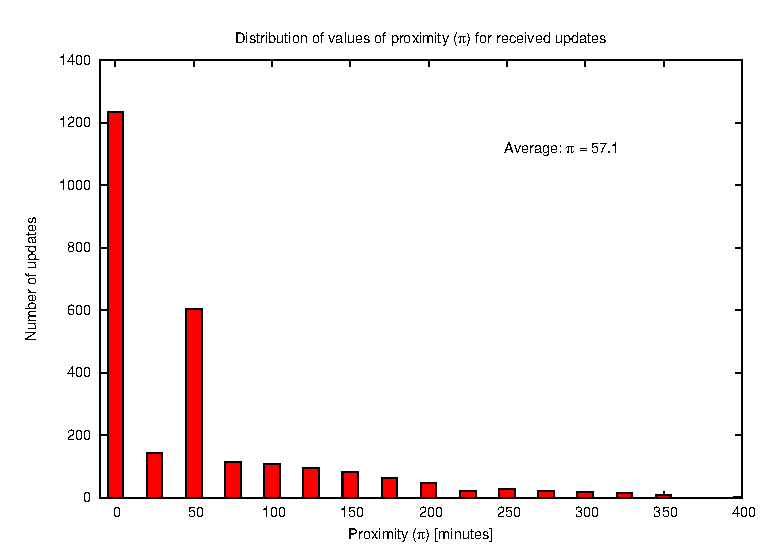
\includegraphics[scale=1.0, angle=0]{figures/vol_pi.eps}
\caption[Distribution of proximity measure $\pi$ for volatile updates received.]
{Distribution of proximity measure $\pi$ for volatile updates received. Peaks occur at 1 minute (44\%) and 60 minutes (23\%) are accounted for by automated inputs from an external microlensing project's agent \citep{tsapras09robonet}.}
\label{fig:vol_pidist}
\end{center}
\end{figure}

\begin{figure}[htbp]
\begin{center}
    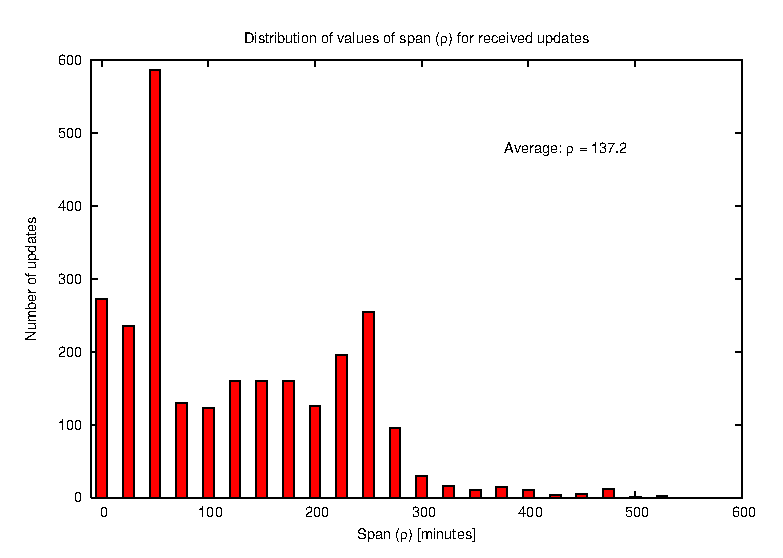
\includegraphics[scale=1.0, angle=0]{figures/vol_span.eps}
\end{center}
\caption[Distribution of span measure $\rho$ for volatile updates received.]
{Distribution of span measure $\rho$ for volatile updates received. There are peaks at 1 hour and 4 hours with cutoff above 5 hours. These are due to a series of automated agent inputs which start either almost immediately or with a 4 hour delay and have flexible timing constraints with 60 minute duration. The 5 hour cutoff is due to longer period flexible groups which set within their observing windows.}
\label{fig:vol_spandist}
\end{figure}

%\begin{figure}[htbp]
%\begin{center}
%    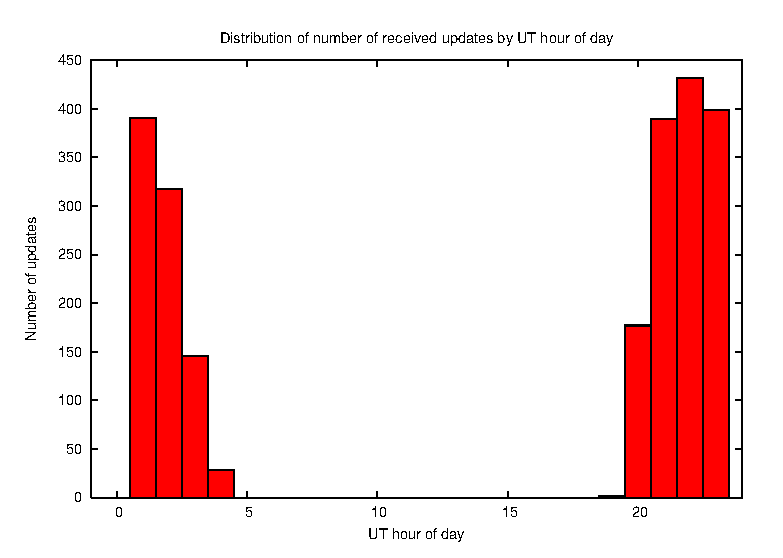
\includegraphics[scale=1.0, angle=0]{figures/vol_ut.eps}
%\end{center}
%\caption[Distribution of UT arrival times of volatile updates received.]
%{Distribution of UT arrival times of volatile updates received.}
%\label{fig:vol_utdist}
%\end{figure}

The recorded event data was processed to count the rate of arrival of events on a per-day basis from the start of the recording period (March 2010) until the end of the period (October 2010). A gap occurred from mid-March until end of April where the recording software was non-functional. From Fig.~\ref{fig:vol_rateplot} we can see that the event rate peaks during June/July with rates of up to 80 events per day. This corresponds to the peak period of galactic bulge observing by the microlensing program. These events are found to consist exclusively of new observations and so add executable time to the schedule. Further analysis Fig.~\ref{fig:vol_execplot} shows that during this period up to 300 minutes (5 hours) of potential observing may be added per night - a significant fraction of the observing night. Unfortunately data showing the total amount of observing available on these nights is not easily obtainable so it is difficult to determine the overall effect on schedules. It is also found from examination of schedule logs that on occasions though many observations are added these will often be in competition with each other for observing time and so cannot in fact all be executed in practice.


\begin{figure}[htbp]
\begin{center}
    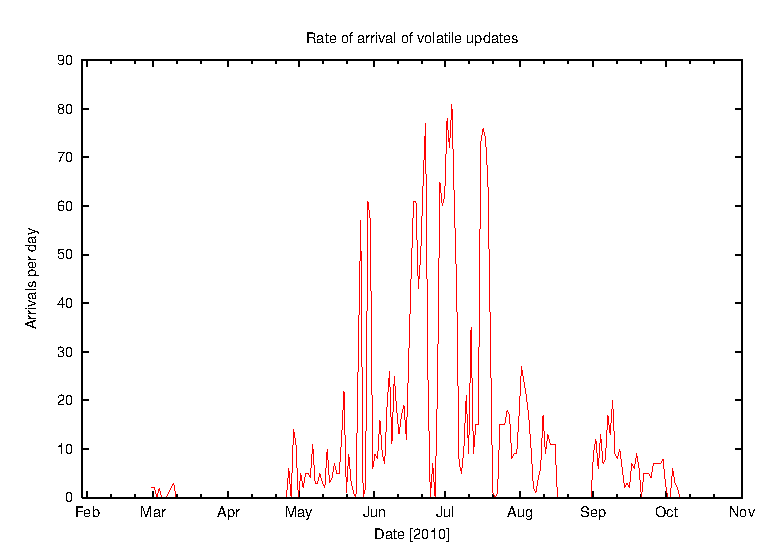
\includegraphics[scale=1.0, angle=0]{figures/volrate.eps}
\end{center}
\caption[Rate of arrival of volatile updates.]
{Rate of arrival of volatile updates. Peak rate of arrivals occurs June-July corresponding to the peak period of galactic bulge observing by the microlensing program with up to 80 events per day.}
\label{fig:vol_rateplot}
\end{figure}

\begin{figure}[htbp]
\begin{center}
    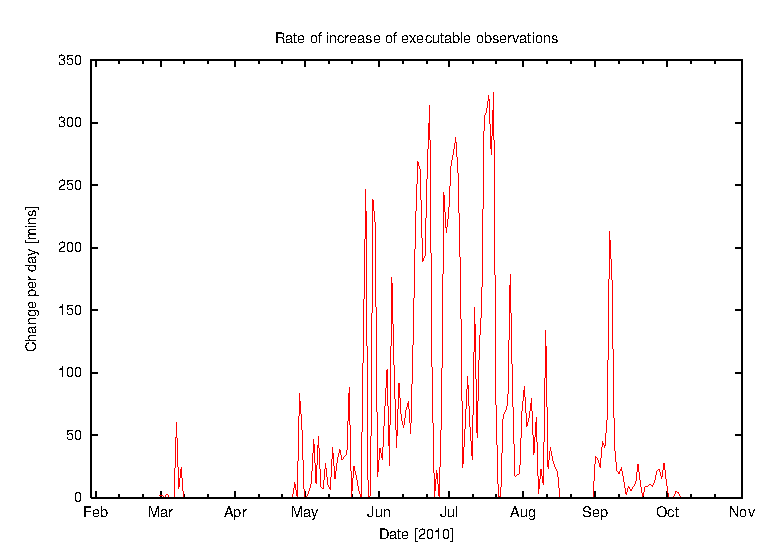
\includegraphics[scale=1.0, angle=0]{figures/volexec.eps}
\end{center}
\caption[Rate of increase of executable observations.]
{Rate of increase of executable observations. During the peak period, up to 300 minutes of new observations arrive per day amounting to around 50\% of the potential observing load.}
\label{fig:vol_execplot}
\end{figure}

\subsection{Simulation}
In order to quantify the effects of volatility it was decided to perform a series of simulations under varying conditions of volatility. The mechanism chosen to implement is the addition to the simulation architecture of a Volatility Scenario Generator (VSG), henceforth denoted by the symbol $\mathcal{V}$ .

A simple volatility generator was devised based on a specified average rate of arrival $(\lambda)$. When the simulator calls on the VSG to generate events over a specified interval (see Fig.~\ref{fig:ss_vgen_flowchart} and Sect.~\ref{ss:sim_ops}) the decision on how many events $(k)$ to generate is calculated based on the poisson distribution $P(k) = \frac{\lambda^k e^{-\lambda}}{k!}$. A random number generator generates a number $r \in [0,1]$. The smallest number $k$ such that $r > P(k)$ is the number of events to be injected.

%%NOTE: Add a simple diagram here to show the method of update as this is quite complicated.
% We use Cached SMP model which uses internally a cached accounting and cached hist models (rather than the usual ASM, HSM which are linked to the external AM and HM) and an enhanced P2C model - this later allows us to add additional groups to a nominated \emph{volatile} proposal. At the start of each run we must, $call clearCaches()$ on the CSMP - this flushes both the casm and cshm, then $clear()$ on the EP2CM. We then create new generous accounts for the volatile proposal. 

%%NOTE: Detail ? When signalled with $fireEvents(t1, t2)$ the simulation time step is guaranteed to advance to \emph{t2} ie nothing can prevent this so we can safely generate all $k$ events in that period at a single moment even though they would naturally appear at intervals and update the EP2CM appropriately as no scheduling decision will be made before \emph{t2} at the earliest. This time might be any of \begin{inparaenum} [\itshape a\upshape)] \item successful completion of a group, \item group completion with internal or external failure reason, \item completion of a background observation or \item completion of an external disruption event. \end{inparaenum}.

\subsection{Investigation into the effect of proximity ($\pi$) on schedule quality}
In this experiment the effect of varying the proximity of groups added via volatility events was investigated. The scoring model was modified to simulate a typical scoring sequence during an observing night. The base groups (those already available via the Phase2 model) produce scores randomly within bounds $[V_{lo}, V_{hi}]$. The groups added via the VSG are specially tagged and have scores set at a predetermined level $V^*$ with a small amount of noise added. 

A total of 7 scheduler models were tested; BDS - a basic despatch scheduler, QLAS - a look-ahead scheduler with horizons of 1, 2 and 4 hours and ELAS - the enhanced look-ahead scheduler with the same three horizons as QLAS (Sect.~\ref{ss:sched_impl}). The environment model was set to a fixed state (good seeing and photometric) for all runs. Simulations were performed as follows:-

\begin{itemize}
\item A set of preliminary simulation runs were performed with each of the selected schedulers but with no volatile events in order to give a baseline.
\item Simulations were then performed with $\pi$ varying logarithmically between 1 minute and 6 hours  in accordance with the limits found from recorded volatility events (Sect.~\ref{sect:volanal}). For each $\pi$ value $\rho$ was chosen from a random distribution in the range $[1, 120]$ minutes. For each $\pi$ value 100 simulations were performed with each of the selected schedulers. The value of $V^*$ is set close to $V_{hi}$ so tagged groups are generally favoured relative to base groups.
\item A third set of simulations were performed with each scheduler in which all of the volatile events were instead fed in at the start before any scheduling took place to allow an upper bound to be set on the potential reward.
\end{itemize}

\subsection{Results}
%The results are presented in Fig.~\ref{fig:vol_pivarlo} and  Fig.~\ref{fig:vol_pivarhi}. These show the reward achieved ($Q_{SU}$) in each run relative to the baselines.   
%For the low scoring events, Fig.~\ref{fig:vol_pivarlo} shows that BDS performs marginally better with the volatile events included - this is accounted by the fact that occasionally a tagged group with a better score than the best available base group is selected and boosts the score marginally. From the same figure we see also that the QLAS perform better than BDS for all horizons in accordance with the results of (Sect.XXX). There is little discernable variation with $\pi$ however. This makes sense in that the QLAS has no better (or at best a marginally better) set of groups to schedule from after the volatile events than without them. We see also a possible slight improvement with increasing $\pi$ in anticipation of results of $V_{hi}$.

The baseline measurements are shown in Table.~\ref{tab:vollohi}. $Q_0$ is the mean value of $Q_{SU}$ measured on simulations with no volatile events. The column labelled $Q_{HI}$ shows the mean results for simulations with \emph{all} the volatile events injected in advance while $\Delta$Q is the difference between these and represents the parameter used to scale the y-axis in the following graphs. As can be seen, in the case of BDS there is a significant improvement when the volatile events are added in. The figures in parenthesis are $\sigma$ values for these means.

Results for the QLAS and ELAS schedulers are displayed in Figs.~\ref{fig:vol_qlas_pi} and \ref{fig:vol_elas_pi}. The quantity plotted on the y-axis is the improvement over the baseline $Q_0$ divided by $\Delta Q$ The results for the various QLAS horizons all show improvement over the baseline values. Most noticably the \emph{rise time} appears to correlate with the horizon length.  QLAS(1) picks up faster than QLAS(2) and QLAS(4). The suggestion here is that the QLAS does not see the changes which occur in a time short compared to its horizon and thus cannot react to them. In fact the QLAS is effectively unavailable for scheduling during the execution of a horizon length sequence, any events occuring in this period are not seen until the end of the execution. However because the events are not synchronized to occur during this period, the QLAS may in fact be at any stage in a sequence's execution so will see some of the tagged groups sooner than 1 full horizon length.

Figures \ref{fig:vol_qe05_pi} through \ref{fig:vol_qe4_pi} show comparisons of the schedulers QLAS and ELAS of the same horizon lengths. Associated statistics are given in Tables.~\ref{b:f127} through \ref{b:f1210}. It is clear that ELAS performs better than QLAS especially at low values of proximity ($\pi$) and that this improvement is greater for schedulers with longer horizons lengths.

% INCLUDE table of lo, hi results for all so can see DeltaV

\begin{table}[htbp]
\begin{center}
\begin{tabular}{|l|l|l|l|}
\hline
\bf{Model} &  $\mathbf{Q_0}$  & $\mathbf{Q_{HI}}$  & $\mathbf{\Delta Q}$ \\
\hline
$B$        & 96 (3)       &  106 (3)      &   10 \\
\hline
$Q_1$      & 102 (2)      &  113 (4)     &   11\\
\hline
$Q_2$      & 105 (4)      &  117 (4)     &  12\\
\hline
$Q_4$      & 108 (4)      &  119 (3)     &  11\\
\hline\hline
$E_1$      & 101.2 (3)    &  114.3 (4)     & 13 \\
\hline
$E_2$      & 105.3 (4)    &  116.5 (4)     &  11\\
\hline
$E_4$      & 107.8 (4)    &  119.3 (3)     &  11\\
\hline
\end{tabular}
\end{center}
\caption[Mean values of $Q_{SU}$ measured using baseline simulations.]
{Mean values of $Q_{SU}$ measured using the baseline simulations. $Q_0$ is the mean value of $Q_{SU}$ measured on simulations with no volatile events. $Q_{HI}$ indicates the  mean value of $Q_{SU}$ measued on simulations with \emph{all} volatile events injected at the start. $\Delta Q$ is the difference and is the parameter used to scale the y-axis in Figs.~\ref{fig:vol_qlas_pi}-\ref{fig:vol_qe4_pi}}.
\label{tab:vollohi}
\end{table}


\begin{figure}[htbp]
\begin{center}
    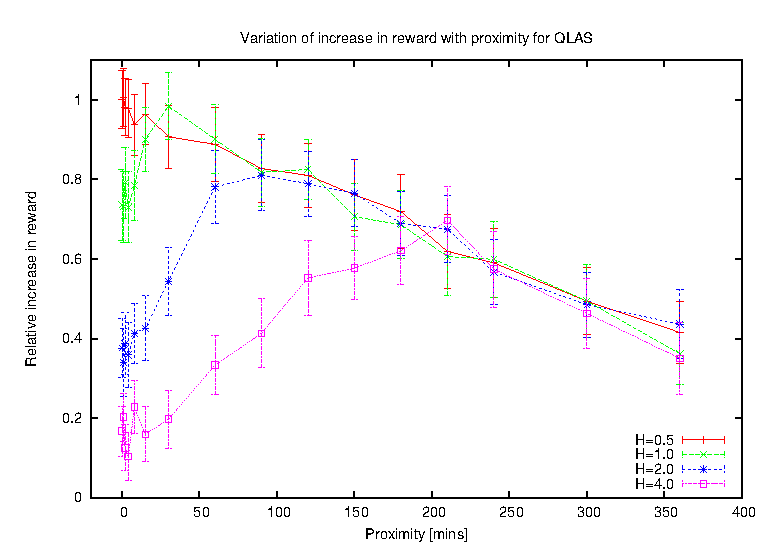
\includegraphics[scale=1.0, angle=0]{figures/vdv.eps}
\end{center}
\caption[Effect of proximity ($\pi$) of volatile events on schedule quality ($Q_{SU}$) for QLAS.]
{Effect of proximity ($\pi$) of volatile events on schedule quality ($Q_{SU}$) for QLAS. All QLAS horizons show improvement over the baseline values. Most noticably the \emph{rise time} appears to correlate with the horizon length. QLAS(1) picks up faster than QLAS(2) and QLAS(4). The suggestion here is that the QLAS does not see the changes which occur in a time short compared to its horizon and thus cannot react to them.}
\label{fig:vol_qlas_pi}
\end{figure}


\begin{figure}[htbp]
\begin{center}
    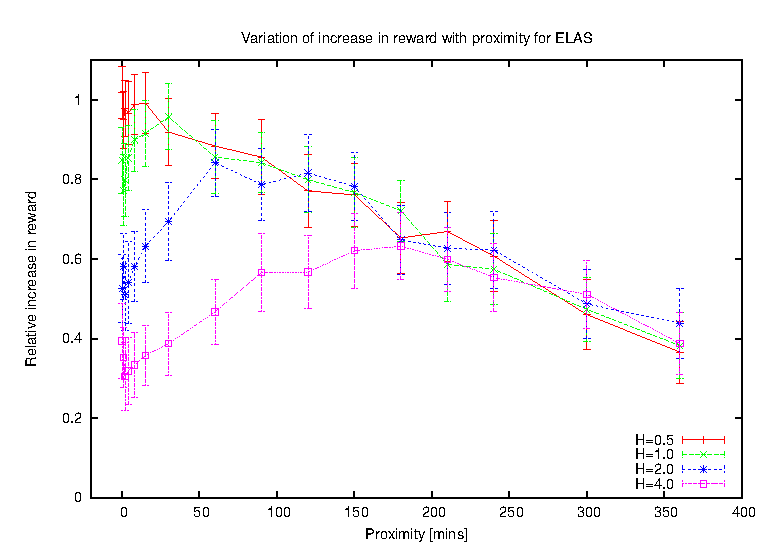
\includegraphics[scale=1.0, angle=0]{figures/edv.eps}
\end{center}
\caption[Effect of proximity ($\pi$) of volatile events on schedule quality ($Q_{SU}$) for ELAS.]
{Effect of proximity ($\pi$) of volatile events on schedule quality ($Q_{SU}$) for ELAS. The ELAS schedulers follow a similar pattern to QLAS but the rise-time is slightly shorter, i.e. the ELAS schedulers react faster to volatile events.}
\label{fig:vol_elas_pi}
\end{figure}

% ev5,1,2,4

\begin{figure}[htbp]
\begin{center}
    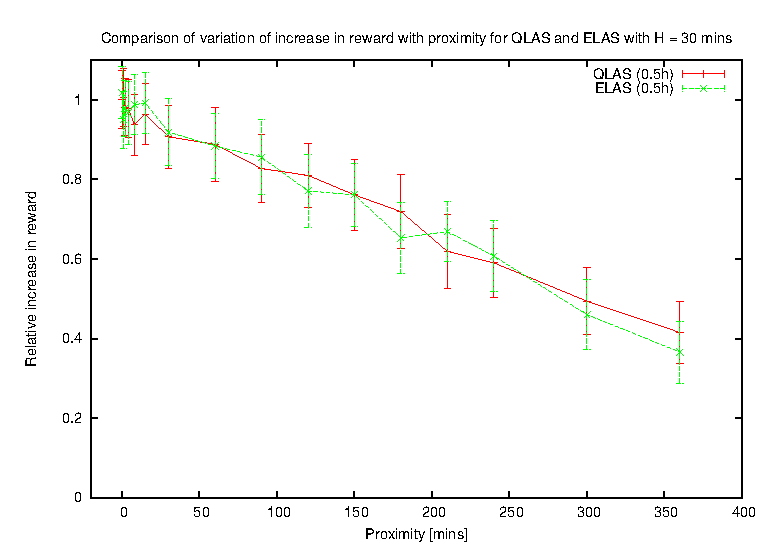
\includegraphics[scale=1.0, angle=0]{figures/evplot_05.eps}
\end{center}
\caption[Comparison of effect of proximity ($\pi$) of volatile events on schedule quality ($Q_{SU}$) for QLAS and ELAS ($H = 0.5h$).]
{Comparison of effect of proximity ($\pi$) of volatile events on schedule quality ($Q_{SU}$) for QLAS and ELAS with $H = 0.5h$.}
\label{fig:vol_qe05_pi}
\end{figure}

\begin{figure}[htbp]
\begin{center}
    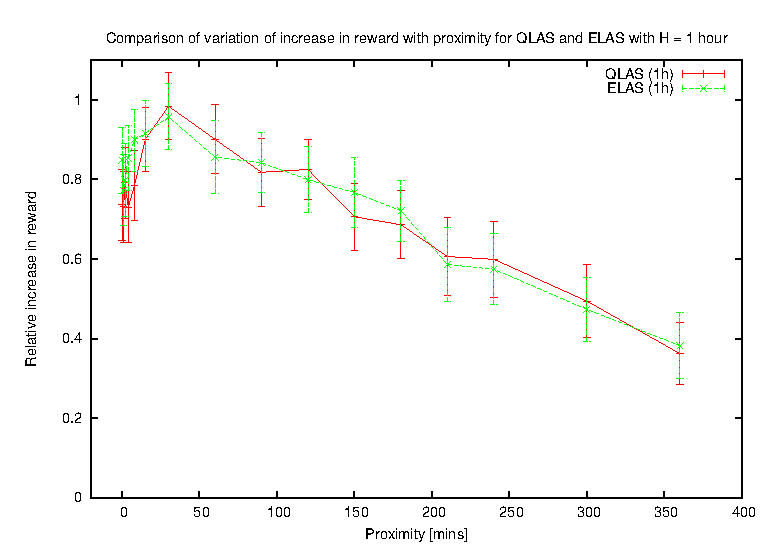
\includegraphics[scale=1.0, angle=0]{figures/evplot_1.eps}
\end{center}
\caption[Comparison of effect of proximity ($\pi$) of volatile events on schedule quality ($Q_{SU}$) for QLAS and ELAS ($H = 1h$).]
{Comparison of effect of proximity ($\pi$) of volatile events on schedule quality ($Q_{SU}$) for QLAS and ELAS with $H = 1h$.}
\label{fig:vol_qe1_pi}
\end{figure}

\begin{figure}[htbp]
\begin{center}
    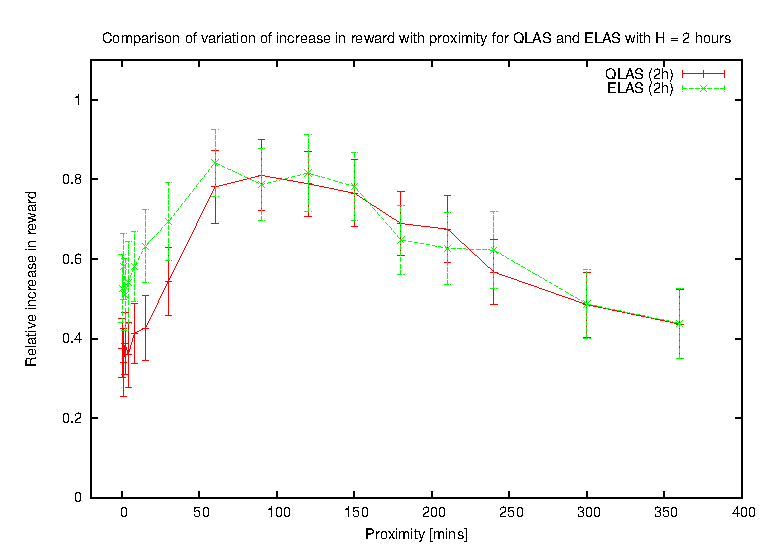
\includegraphics[scale=1.0, angle=0]{figures/evplot_2.eps}
\end{center}
\caption[Comparison of effect of proximity ($\pi$) of volatile events on schedule quality ($Q_{SU}$) for QLAS and ELAS ($H = 2h$).]
{Comparison of effect of proximity ($\pi$) of volatile events on schedule quality ($Q_{SU}$) for QLAS and ELAS with $H = 2h$. This plot shows some improvement in quality by ELAS over QLAS at lower proximity.}
\label{fig:vol_qe2_pi}
\end{figure}

\begin{figure}[htbp]
\begin{center}
    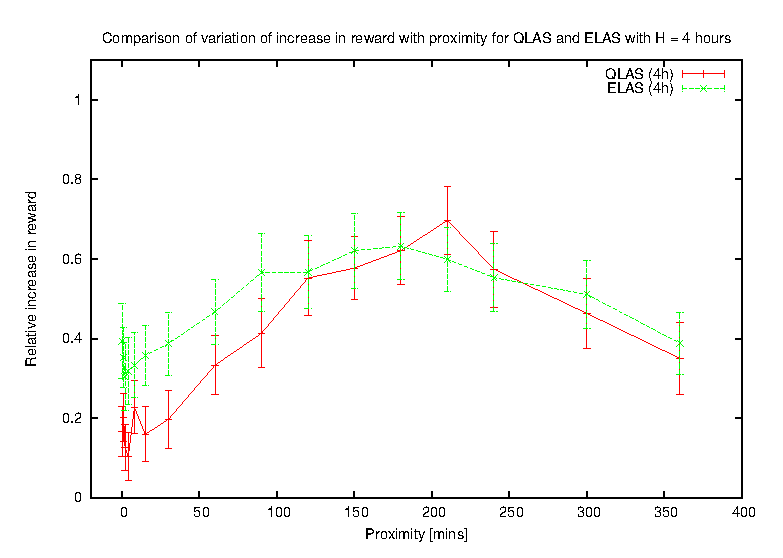
\includegraphics[scale=1.0, angle=0]{figures/evplot_4.eps}
\end{center}
\caption[Comparison of effect of proximity ($\pi$) of volatile events on schedule quality ($Q_{SU}$) for QLAS and ELAS ($H = 4h$).]
{Comparison of effect of proximity ($\pi$) of volatile events on schedule quality ($Q_{SU}$) for QLAS and ELAS with $H = 4h$. This plot shows the most improvement in quality by ELAS over QLAS at low proximity.}
\label{fig:vol_qe4_pi}
\end{figure}

\subsection{Summary and conclusions}
Embedded instrumentation was used to record changes to the Phase 2 ODB, termed volatile events. Some simple metrics were designed with which to characterize these events. It was found that at busy times up to 50\% of the nights potential observations can arrive after the start of night's observing.

In simulation experiments it was found that for any given look-ahead horizon H there was an optimum value of proximity (one of the characterization metrics) at which the highest relative improvement occured. This was found to be related to H. An enhanced look-ahead scheduler, ELAS which included a sequestration policy was introduced and this was seen to yield further improvement in schedule quality. The effectivenss of ELAS relative to QLAS was seen to increase with increasing horizon length.
